\documentclass[a4paper,12pt]{report}

\usepackage[utf8]{inputenc}
\usepackage[T1]{fontenc}
\usepackage{array}
\usepackage{amsmath}
\usepackage[english]{babel}
\usepackage{graphicx}
\usepackage[a4paper]{geometry}
\usepackage[colorlinks=true,urlcolor=blue,linkcolor=blue]{hyperref}
\usepackage{url}
\usepackage[nottoc,numbib]{tocbibind}
\usepackage{color}
\usepackage{epstopdf}
\usepackage{xcolor}
\usepackage[backend=biber,style=phys]{biblatex}
\usepackage[capbesideposition={right,center}]{floatrow}
\usepackage{lipsum}

\addbibresource{../Bibliography.bib}

\makeatletter
	\renewcommand{\thechapter}{\Roman{chapter}}
\makeatother

\floatsetup[table]{style=plaintop}

\begin{document}

\chapter{Dynamics and optical control of an individual Cr spin in a CdTe QD\label{CrDyn}}
	
	We successfully included a single Cr atom in CdTe quantum dot, and were able to probe them optically. We evidenced a strong spin-to-strain coupling for the Cr, particularly promising for the development of hybrid spin-mechanical systems and coherent mechanical driving. To be able to perform these experiments, the first key steps are the possibility to prepare the spin of a single magnetic atom and probe its dynamics.
	
	First, the dynamics under optical excitation was accessed using photon correlation techniques. Auto-correlation of the photons emitted by the QD under continuous optical excitation reveals fluctuations of the localized spin with a timescale in the 10 ns range. Cross-correlation gives quantitative transfer time between Cr spin states.
	
	In the second part, we demonstrate the possibility to prepare the Cr spin using resonant optical pumping. Monitoring the time dependence of the intensity of the resonant fluorescence of the quantum dot during this process permits to probe the dynamics of the optical initialization of the Cr spin. Using resonant excitation, we identify phonon-mediated transfer channels for the Cr spin under excitation via phonon-mediated hole-Cr spin flip-flop. Heating of the Cr spin by non-equilibrium acoustic phonons is also evidenced.

	Finally, we demonstrate that, under a resonant single-mode laser field, the energy of any spin state of an individual Cr atom can be independently tuned by using the optical Stark shift effect.
	
	\section{Probing the spin fluctuations of the Cr\label{ProbeSpinFluc}}
	
%	In order to probe the X-Cr dynamics under excitation, we performed auto-correlation of the photoluminescence (PL) intensity emitted by individual lines of an isolated Cr-doped QD to probe the dynamics of the magnetic atom under continuous wave (CW) optical excitation.
	
	The easiest way to look at the Cr spin dynamics under continuous wave (CW) optical excitation is to probe the statistics of time arrivals of the photons emitted in a given PL peak. To do that, we used a Hanbury Brown and Twiss (HBT) setup with a time resolution of 0.8 ns. In these start-stop experiments, the detection of the first photon indicates by its energy and polarization that the Cr spin has a given orientation. The probability of detection of a second photon with the same energy and polarization is proportional to the probability of conserving this spin state. For processes fast compared to the inverse of the count rate, this measure gives a good approximation of the autocorrelation function $g^{(2)}(\tau)$.
	
	\begin{figure}[h!]
	\fcapside{\caption{Auto-correlation of the PL intensity collected in circular polarization on the X-Cr lines (1), (4) and (5) and compared with the auto-correlation of the exciton in a non-magnetic QD (black line). The curves are shifted for clarity. For line (1), the auto-correlation is also recorded under a transverse magnetic field $B_x = 0.42$ T (blue line).}\label{AutocorExpCr}}	
	{\begin{center}
		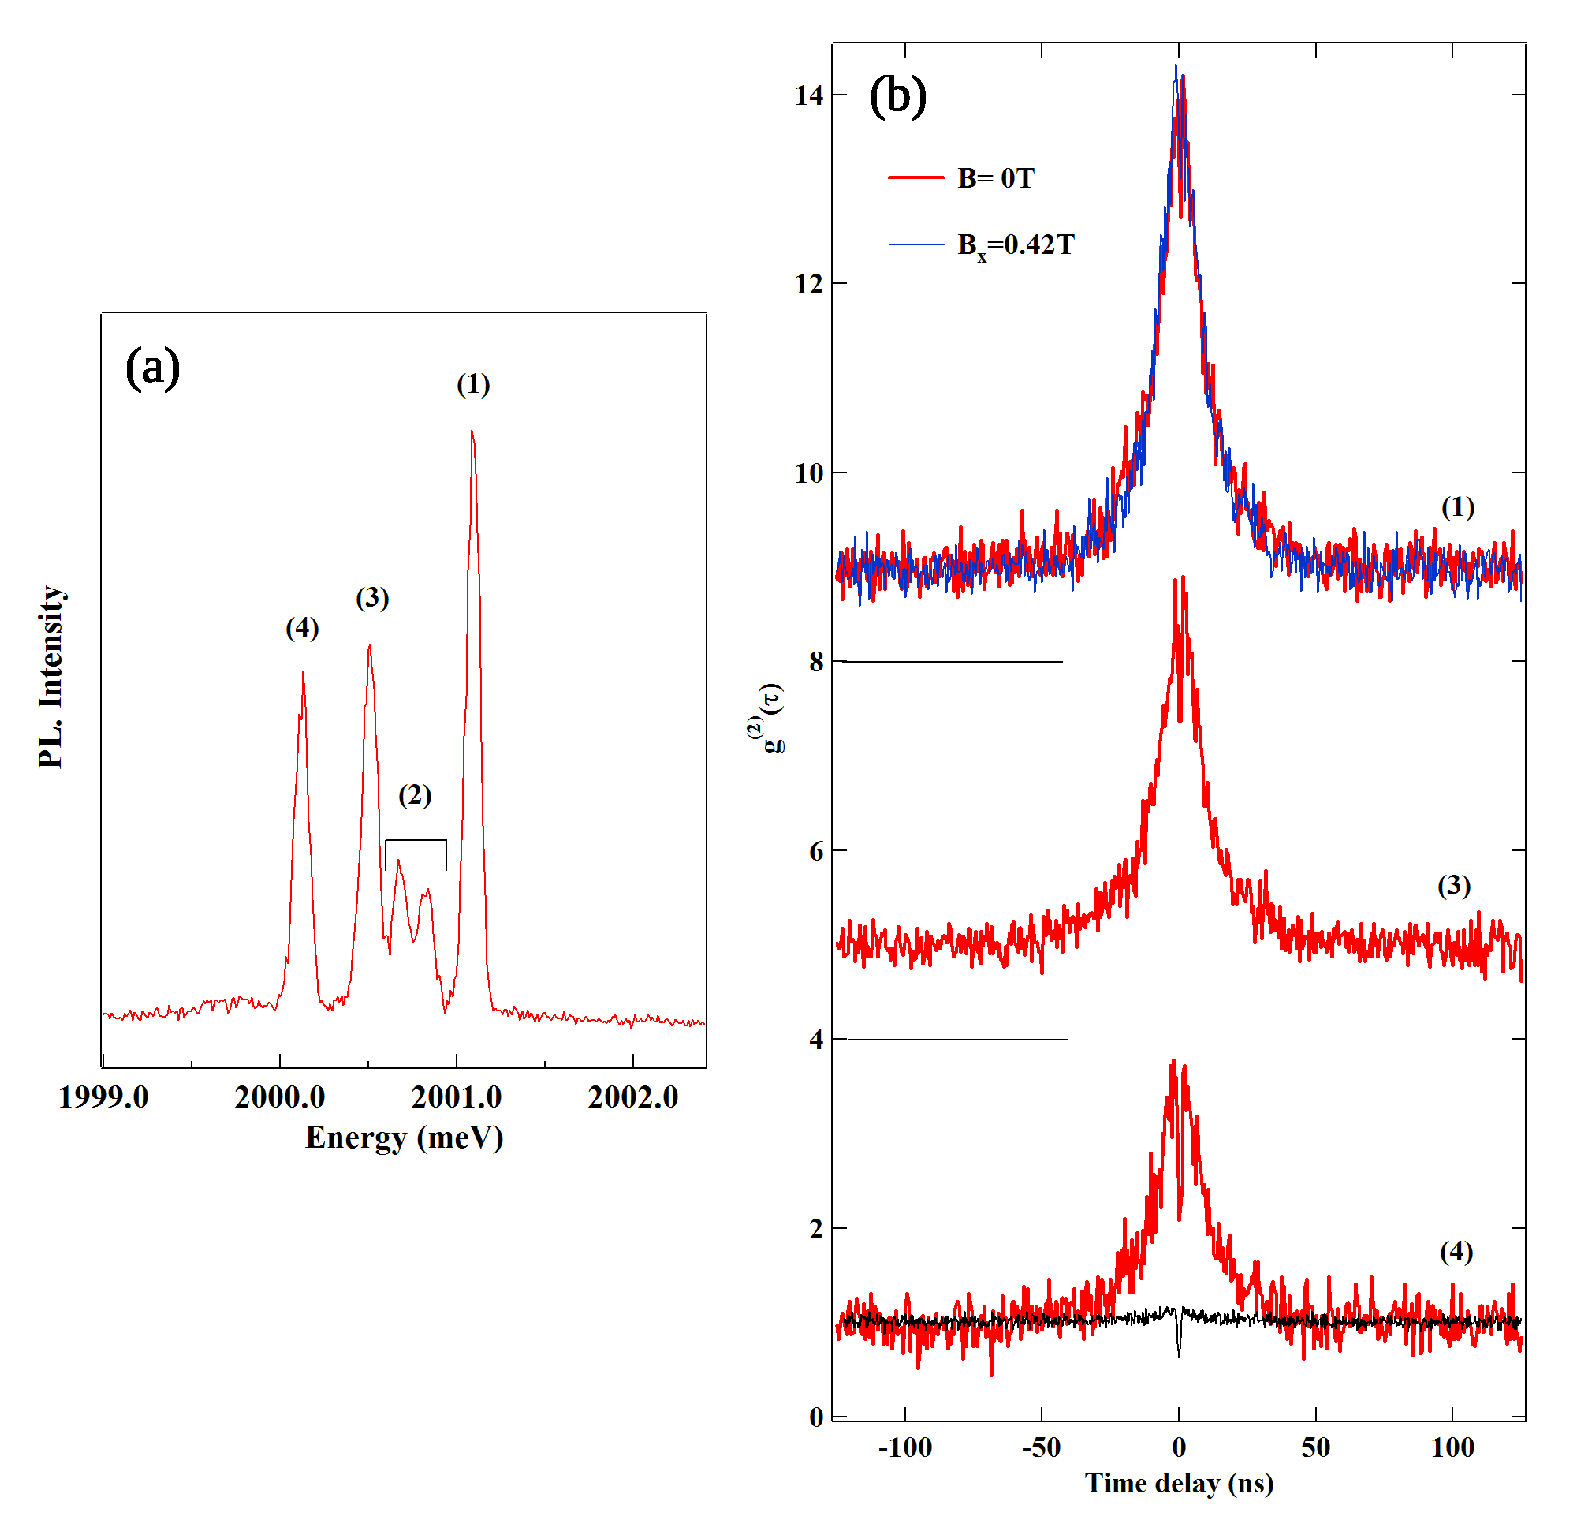
\includegraphics[width=7cm]{Pictures/AutocorPeaks.eps}
	\end{center}}
	\end{figure}	
	
	The experiments were performed on QD2, presented in Fig.~IV.1%~\ref{SpectraX}
. The PL of QD2 is reported in the inset of Fig.~\ref{AutocorExpCr}. This QD presents a large splitting between each peaks, making the probing of a single state easier. Fig.~\ref{AutocorExpCr} shows g$^{(2)}(\tau)$ for the lines (1), (4) and (5) recorded in circular polarization. These signals are compared with the auto-correlation obtained for the PL of a non-magnetic QD (black line) which is characteristic of a single-photon emitter with a dip (anti-bunching) at short delays. The width of the anti-bunching is given by the lifetime of the emitter and the generation rate of excitons and its depth is limited by the time resolution of the HBT setup. As illustrated in Fig.~\ref{AutocorExpCr}, typical non-magnetic CdTe/ZnTe QDs do not present any significant bunching induced by charge fluctuations \cite{QDAutocor,IndistPhoton}. A similar auto-correlation on a X-Cr PL line still presents a reduced coincidence rate near zero delay, but it is mainly characterized by a large photon bunching with a full width at half maximum (FWHM) in the 20 ns range. This large bunching reflects an intermittency in the emission of a given line of the QD coming from fluctuations of the Cr spin in a 10 ns timescale as it will be confirmed by cross-correlation measurements.

		The amplitude of the bunching reaches 5 for line (1) and is slightly weaker for the lower energy lines. In a simple picture of blinking where the selected QD line can be either in a state ON (populated) or OFF (empty), the amplitude of the bunching is given by $\Gamma_{OFF}/\Gamma_{ON}$, with $\Gamma_{ON}$ the transition rates from OFF to ON, and $\Gamma_{OFF}$ the one from ON to OFF~\cite{SubnanoSpectDiff}. An amplitude of bunching larger than 1 is then expected in a multilevel spin system where, after a spin relaxation, multiple spin-flips are usually required to come back to the initial state ($\Gamma_{ON}<\Gamma_{OFF}$). Let us also note that the bunching signal is not affected by a weak transverse magnetic field ($B_x=0.42$ T in Fig.~\ref{AutocorExpCr}). This confirms the presence of a large strain induced magnetic anisotropy $D_0$ which splits the Cr and X-Cr states and blocks their precession in a magnetic field.
		
	\begin{figure}[h!]
	\fcapside{\caption{Auto-correlation of the PL intensity recorded in circular polarization on the high energy X-Cr line (1) for different excitation powers. The inset shows the corresponding FWHM of the bunching signal versus excitation power.}\label{AutocorPW}}	
	{\begin{center}
		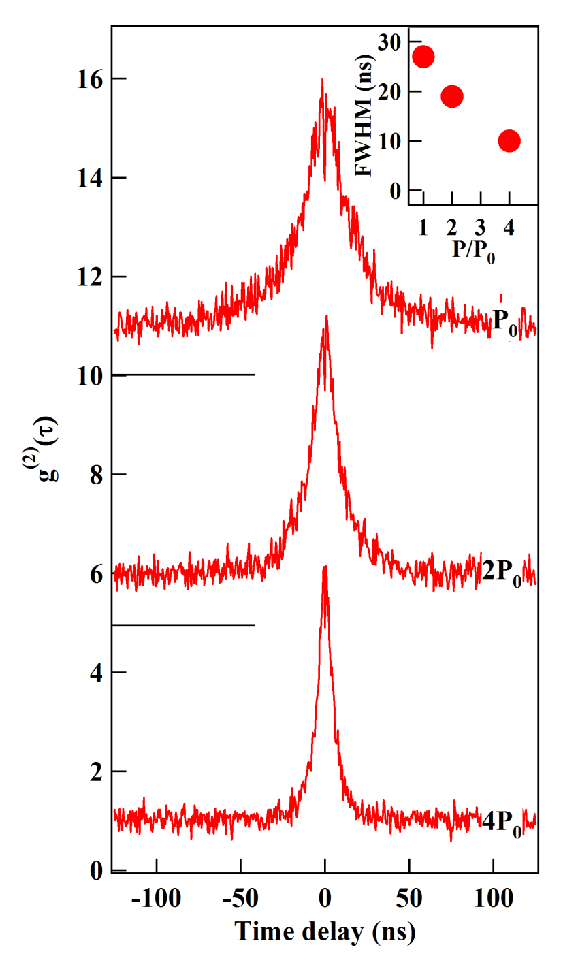
\includegraphics[width=6cm]{Pictures/AutocorPw.eps}
	\end{center}}
	\end{figure}
	
	The observed spin dynamics depends on the optical excitation power. Increasing the excitation power significantly reduces the width of the bunching (Fig.~\ref{AutocorPW}), linked to an increase of the Cr spin fluctuations. Within the X-Cr complex, the electron-Cr exchange interaction and the hole-Cr exchange interaction in the presence of heavy-hole/light-hole mixing can both induce spin-flips of the Cr. Though weak, the probability of such spin flips increases with the occupation of the QD with an exciton and dominates the spin dynamics in the high excitation regime required for the photon correlation measurements.
	
	\begin{figure}[h!]
	\begin{center}
		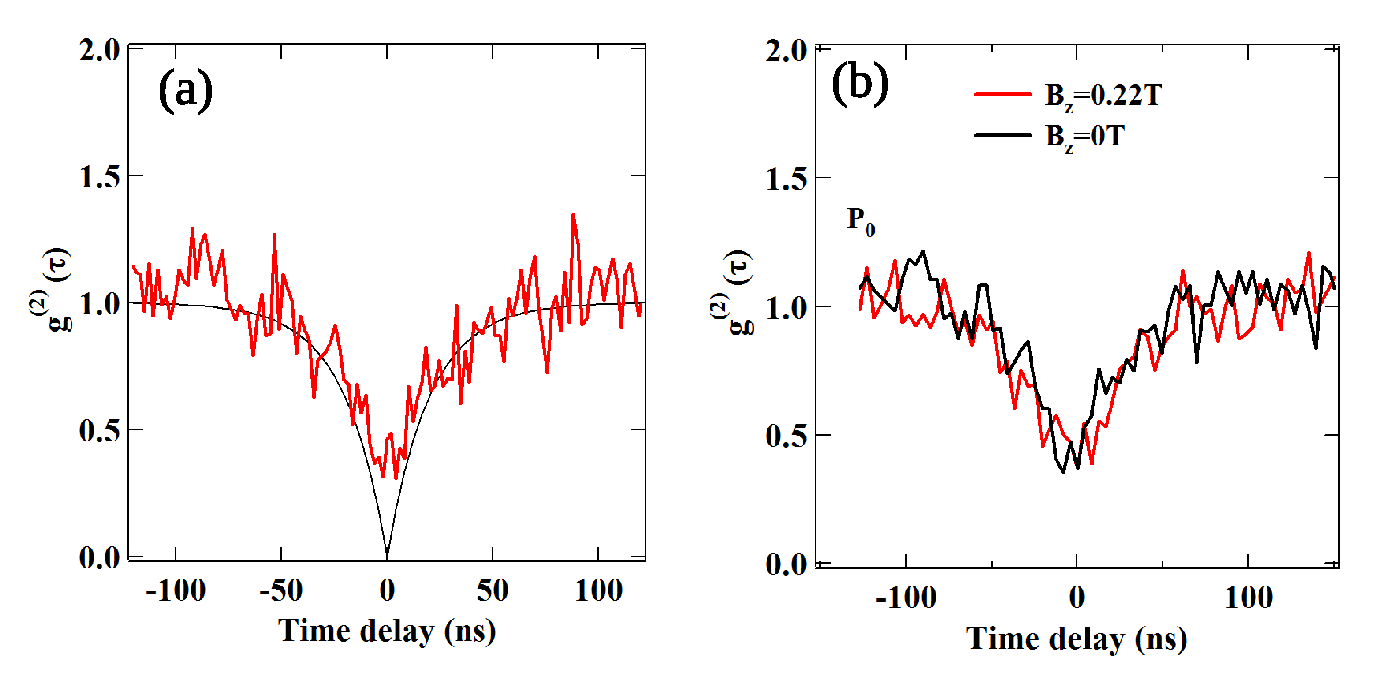
\includegraphics[width=10cm]{Pictures/CrosscorFit+B.eps}
	\end{center}
	\caption{(a) Correlation signal of the PL intensity of lines (1) and (4) recorded in the same circular polarization (cross-correlation) for three different excitation powers. The curves are shifted for clarity. The black line is an exponential fit with a characteristic time $\tau=20$ ns. (b) Longitudinal magnetic field dependence of the cross-correlation signal obtained at low excitation power.}
	\label{Crosscor}
	\end{figure}
	
	The excitation power dependence shows that the measured width of the bunching is not limited by the intrinsic Cr spin relaxation time $\tau_{Cr}$. This gives a lower bound for $\tau_{Cr}$ in the 20 ns range. A shorter value would impose, at low excitation intensity, faster spin fluctuations than observed experimentally. The Cr spin relaxation time is ultimately controlled by the interaction with acoustic phonons and can depend on the optical excitation through the generation of non-equilibrium acoustic phonons during the relaxation of injected carriers~\cite{PhotocarrierSpinHeat, EnTransPhotocarrierMn}. It is however difficult to probe this spin lattice coupling in autocorrelation measurement: the large photon count rate needed for this experiment means that the QD is occupied by an exciton most of the time.
	
	To analyze more in detail the Cr spin relaxation channels, cross-correlation measurements were performed on the PL emitted by the high energy and the low energy lines in the same circular polarization. The cross-correlation shows a large anti-bunching with a FWHM in the 10 ns range and $g^{(2)}(0) \approx 0.3$ (Fig.~\ref{Crosscor}(a)). Whereas the auto-correlation probes the probability for the Cr spin to be conserved, this cross-correlation is a probe of the spin transfer time between the spin states $S_z=+1$ and $S_z=-1$. As for the auto-correlation, the cross-correlation strongly depends on the excitation power. At weak excitation, a spin transfer time of about 20 ns is observed. It is accelerated with the increase of the excitation power (Fig.~\ref{Crosscor}(a)). This transfer time could be controlled by anisotropic in-plane strain which couples Cr spin states separated by two units through an additional term $E(S_x^2-S_y^2)$ in the Cr fine structure Hamiltonian~\cite{LafuenteCrQD}. However, even at low excitation power, the measured transfer time is not affected by a longitudinal magnetic field (Fig.~\ref{Crosscor}(b)). This shows that for such QD the strain anisotropy term $E$ is weak and is not the main parameter controlling the transfer time between the states $S_z=\pm1$. The spin transfer time is dominated by spin-flips induced by the exciton/Cr interaction.
	
	This fast transfer time is an indication of efficient carrier-Cr spins flip-flop, an interaction with optically injected acoustic phonons, or both. However, it is hard to extract precise informations from the auto-correlation and cross-correlation experiments only. In order to delve into more details, we have to use more precise tools.
	
	\section{Resonant optical pumping of a Cr spin\label{ResOptPump}}
		
	A more efficient way to probe the dynamics of a Cr spin under excitation or in the dark is to perform resonant optical pumping. To do that, we tuned a laser in resonance with one of the transition of the QD: an exciton can only be injected if the Cr spin is in the resonantly excited state. If the intraband relaxation time of the X-Cr complex is smaller than the one of the Cr alone ($\tau_{Cr} > \tau_{X-Cr}$), the Cr may undergo spin-flips after an absorption, progressively decreasing the population of the resonantly excited state. Once it is empty, the resonant laser cannot injects exciton in the QD anymore. A signature of the pumping can be detected by looking at the cross-polarized PL of the low energy line of the dot, after a spin-flip of the exciton. In this configuration, both the excitation and the detection are done on the same Cr spin state. It supposes that the spin flip time of the exciton in presence of Cr is smaller than the relaxation time of the Cr in the excited state $\tau_{X-Cr}$. This process is illustrated on the inset of Fig.~\ref{PumpPres} for an excitation of $|S_z = -1, X_z = -1 \rangle$ state.
	
	\begin{figure}[h!]
	\begin{center}
		\includegraphics[width=14.7cm]{Pictures/PumpPres.png}
	\end{center}
	\caption{Low temperature PL spectra of QD2 exciton in cross-linearly polarized excitation and detection at B = 0T. No contribution of the charge excitons was found. Inset: Schematic of the energy levels in a Cr-doped QD and configuration of excitation/detection for resonant optical pumping.
%	The ground states $S_z = 0$, $\pm1$ are split by the magnetic anisotropy $D_0 S_z^2$. In the excited state (X-Cr), the exchange interaction with the bright exciton ($|\pm1\rangle$) split the states $S_z = \pm1$.
}
	\label{PumpPres}
	\end{figure}
	
%	The dynamics of the X-Cr system can be modified by the presence of supplementary carriers in the QD. To study this dynamics properly, we therefore need a QD in which it is uncommon to have more carriers than a single exciton. QD2 presents such characteristic. Its spectra, shown on a large energy range on Fig.~\ref{PumpPres}, has no contribution of the charged exciton states. Even at high power, we were not able to observe a contribution of the biexciton.
%	
	To perform resonant optical pumping of the Cr spin, we developed a two wavelengths pump-probe experiment. A circularly polarized single mode laser (\emph{resonant pump}) tuned on a X-Cr level is used to pump the Cr spin (i.e., empty the spin state under resonant excitation). Then, a second laser, tuned on an excited state of the QD (\emph{quasi-resonant probe}), injects excitons independently of the Cr spin $S_z$ and drives the Cr to an effective spin temperature where the three ground states $S_z=0, \pm1$ are populated~\cite{LafuenteCrQD}. By recording the PL of a X-Cr lines in circular polarization under this periodic sequence of excitation, we can monitor the time evolution of the population of a given Cr spin state.
	
	\begin{figure}[h!]
	\begin{center}
		\includegraphics[width=13cm]{Pictures/ExperimentSchema.png}
	\end{center}
	\caption{Schematic view of the micro-spectroscopy set-up used for the time-resolved optical pumping experiment. The monomode laser is a dye laser, cross-circularly polarized and tuned on resonance with the studied dot transition, acting as the pump. The other dye laser is tuned on an excited state of the dot, acting as the probe. Both beam splitters are non-polarizing.}
	\label{PumpExpSetup}
	\end{figure}	
		
	Fig.~\ref{PumpExpSetup} shows our experimental set-up. The intensity of both lasers can be switched ON and OFF with accousto-optic modulators with a time response of about 10 ns. This permits to create trains of pulses with different duration and delay. The two lasers are focused on the sample with a microscope objective. A high index ($n \approx 2.5$) Solid Immersion Lens (SIL) is also mounted on the sample surface, to increase the spatial resolution and the collection of photons emitted by the QD. The emitted light is dispersed and filtered by a double monochromator and is then collected with an avalanche photodiode with a time resolution of about 350 ps.
	
	\begin{figure}[h!]
	\begin{center}
		\includegraphics[width=13cm]{Pictures/PumpResults.png}
	\end{center}
	\caption{(a) PL transients recorded in circular polarization on line (3) and on line (4) (as defined in the inset) under the resonant (pump on (1)) and quasi-resonant optical excitation sequences displayed at the bottom. Inset: PL of X-Cr and configuration of the resonant excitation and detection. (b) and (c): Energy detuning dependence of resonant PL intensity ($I_1$, at the beginning and $I_2$, at the end of the pump pulse) and of the corresponding normalized amplitude of pumping transient $\Delta I/I_2 = (I_1-I_2)/I_2$.}
	\label{PumpingExp}
	\end{figure}		
		
	The main features of the optical pumping experiment are presented in Fig.~\ref{PumpingExp} (a). The QD is excited on the high energy state of X-Cr with $\sigma-$ photons (X-Cr state $|S_z = -1, X_z = -1\rangle$), only creating an exciton in the dot if the Cr spin is $S_z = -1$. %This excitation can only create an exciton in the dot if the Cr spin is $S_z=-1$. An absorption followed by possible spin-flips of the Cr in the exchange field of the exciton progressively decreases the population of $S_z=-1$.
After this pumping sequence, the resonant pump is switched off and followed by the non-resonant probe.

	A clear signature of the optical pumping appears on the time evolution of the PL intensity of the low energy bright exciton line (4). The PL of this line during the probe pulse, recorded in opposite circular polarization with the resonant pump, depends on the population of $S_z=-1$. It strongly differs between the two pump-probe sequences, where the resonant pump is either on or off. The difference of intensity at the beginning of the probe pulse is a measurement of the efficiency of the pumping. The PL transient during the probe pulse corresponds to a destruction of the non-equilibrium population distribution prepared by the pump. As expected for an increase of the Cr spin temperature, the population of the ground spin state $S_z=0$ decreases during the probe pulse. This decrease directly appears in the time evolution of the amplitude of the central X-Cr lines during the probe pulse (Det. (3) in Fig.~\ref{PumpingExp} (a)). The decrease of the population of $S_z=0$ during the probe pulse shows that the population of $S_z=-1$ has been partially transferred to $S_z=0$ during the resonant pumping sequence. This will be described in more details in Sec.~\ref{PhononHeat}.
	
	A more direct way to probe the optical pumping speed and efficiency is to monitor the time evolution of the PL during the resonant excitation by the pump pulse. Under resonant excitation on the high energy X-Cr line, an exciton spin-flip with conservation of the Cr spin can produce a PL on the low energy line~\cite{ClaireOptInit}. This experiment configuration is illustrated in the inset of Fig.~\ref{PumpPres}. In this process, the exciton flips its spin by emitting (or absorbing) an acoustic phonon. Such spin-flip is enhanced by the large acoustic phonon density of states at the energy of the inter-level splitting induced by the exchange interaction with the Cr spin which act as an effective magnetic field~\cite{ExcSpinRelaxQD, ExcSpinDecay}. The resulting weak resonant PL signal depends on the occupation of the Cr state $S_z=-1$ and is used to monitor the time dependence of the spin selective absorption of the QD.
	
	The time evolution of the PL of the low energy line of X-Cr under an excitation on the high energy line is presented in Fig.~\ref{PumpingExp} (a) for two different pump-probe sequences: probe on and probe off. When the probe laser is on, a large effective Cr spin temperature is established before each pumping pulse. The amplitude of the resonant PL is maximum at the beginning of the pump pulse ($I_1$) and progressively decreases. A decrease of about 80\% is observed with a characteristic decay time in the tens of $ns$ range. When the probe laser is off, the initial amplitude of the PL transient during the pump pulse is significantly weaker. This decrease is a consequence of the conservation of the out of equilibrium Cr spin distribution during the dark time between two consecutive pumping pulses.
	
	The steady state resonant PL intensity reached at the end of the pump pulse ($I_2$) depends on the optical pumping efficiency. It is controlled by the ratio of the spin-flip rate for the Cr spin in the exchange field of the exciton and the relaxation of the Cr spin in the empty dot, except for optically created acoustic phonons. However, even with cross-circularly polarized excitation/detection, this steady state PL can also contain a weak contribution from an absorption in the acoustic phonon sideband of the low energy line~\cite{BesombesAccPhon}. Fig.~\ref{PumpingExp} (b) presents the amplitude of the resonant PL detected on the low energy line for a detuning of the pump around the high energy line. A resonance is observed in the initial amplitude $I_1$ of the PL. It reflects the energy dependence of the absorption of the QD. A small decrease of the steady state PL $I_2$ is also observed at the resonance. As displayed in Fig.~\ref{PumpingExp} (c), the corresponding normalized amplitude of the pumping transient, $(I_1-I_2)/I_2$, presents a clear resonant behaviour demonstrating the excitation energy dependence of the optical pumping process. The width of the resonance ($\sim 100\mu eV$) is the width of the QD's absorption broadened by the fluctuating environment~\cite{SubnanoSpectralDiff}.
	
	\begin{figure}[h!]
	\caption{Optical pumping under a CW probe at $E = 2004$ meV. (a) Pumping on line (1) and detecting on line (4). (b) Pumping on line (4) and detecting on line (1).}
	\label{ContProbe}
	{\begin{center}
		\includegraphics[width=10.8cm]{Pictures/ContProbe.eps}
	\end{center}}
	\end{figure}
	
	A signature of the optical pumping can also be observed without modulating the probe (probe ON all the time). We did the experiment in two configurations, presented on Fig.~\ref{ContProbe}: either exciting resonantly on line (1) (high energy line, $|S_z = -1, X_z = -1 \rangle$ in $\sigma-$ polarization) and detecting on line (4) (low energy line, $|S_z = -1, X_z = +1 \rangle$), or the opposite (exciting at low energy and detecting at high energy). The signal was detected in $\sigma_{cross}$ configuration. When the pump pulse is turned on the high energy peak, we can see the same transients as shown in Fig.~\ref{PumpingExp} (a): a first, quick increase followed by a slower decrease. The pumping transient seems smaller due to the high background signal created by the continuous probe. When the pulse is turned off, the  PL decreases quickly, followed by a slow increase during about 200 ns before coming back at the intensity it has before the pumping. This is the same transient as the one observed on the probe pulse in Fig.~\ref{PumpingExp} (a).
	
	The complimentary evolution happens when we pump on the low energy line (4) and detect on the high energy line (1). In this case, when the pumping laser is turned on, we first observe a decrease with a time scale of about 100 ns, corresponding to the pumping of the state $S_z = -1$. No increase of intensity is detected because the resonantly excited state ($|S_z = -1, X_z = +1 \rangle$) is at lower energy than the the monitored state ($|S_z = -1, X_z = -1 \rangle$). Therefore, no exciton population transfer can occur between these states, and the observed decrease corresponds only to a decrease of the population of the Cr spin state $S_z = -1$. After this decrease, a steady state remains, with a low PL intensity. The PL intensity then increases slowly in a 200 ns timescale, when the population is restored by the non-resonant laser, caused by the same process as the second transient on Fig.~\ref{ContProbe} (a).
	
	To summarize, we demonstrated the possibility to optically pepare the spin of a Cr atom embedded in a QD via resonant optical pumping, and the ability to probe the pumped Cr state after a exciton spin-flip. This preparation can be used to study the dynamic of the Cr spin in different configuration, and open the possibility to study other phenomena than the autocorrelation alone.

	\section{Dynamics of a Cr spin under optical excitation}
	
	We begin looking at the evolution of the pumping and heating transients with the excitation power. As for the autocorrelation, it permits to probe of the dynamic of the X-Cr system under excitation.
	
	\begin{figure}[h!]
	\begin{center}
		\includegraphics[width=14cm]{Pictures/PWProbe.eps}
	\end{center}
	\caption{PL transients measured on line (4) while pumping on line (1) at $P_{pump} = 250$ $\mu$W (red) or without pumping (dark). (a) $P_{probe} = 125 $ $\mu$W. (b) $P_{probe} = 250 $ $\mu$W. (c) $P_{probe} = 500 $ $\mu$W.}
	\label{PWProbe}
	\end{figure}
	
	We first studied the evolution of the heating transient with the probe laser. The results are presented on Fig.~\ref{PWProbe}. The first noticeable evolution is the expected increase of the PL intensity during the probe pulse, proportional to the increase of the probe power. More interestingly, we observe that the speed of this spin heating process depends on the intensity of the probe laser. The probe pulse last for about 500 ns, and, for a laser power of 125 $\mu$W, the non equilibrium population distribution is not completely destroyed at the end of it (Fig.~\ref{PWProbe} (a)). The transient reduces to about 200 ns for a laser power of 500 $\mu$W. One cause of the speeding of the heating process may be the higher rate of carriers injection. Along with the optically created acoustic phonons, the interaction with the excitons also heat the Cr spin. The probe inject excitons at high energy in the QD, interacting with the Cr independently of its spin state. A higher number of injected high energy carriers therefore leads to a quicker destruction of the non equilibrium state created by the pump pulse. However, other phenomena, such as the coupling of the Cr spin with out of equilibrium phonons, can cause this spin heating.
	
	\begin{figure}
	\fcapside{\caption{Detail of the PL transient measured during the resonant pump pulse on line (1) for a power $P_{probe} = 250$ $\mu$W. The detection was done on line (4). The exponential fit (green) gives a characteristic time of $\tau_{pump} = 60$ ns. The inset presents the evolution of $\tau_{pump}$ as a function of the pumping laser power.}\label{PWPump}}
	{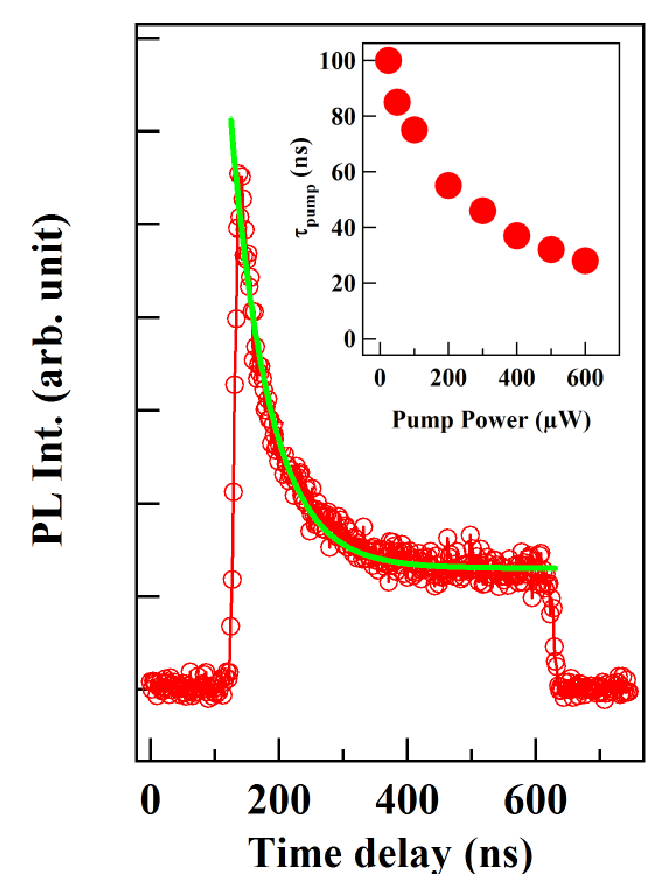
\includegraphics[width=6cm]{Pictures/PWPump.eps}}
	\end{figure}
	
	Study of the evolution of the pumping transient as a function of the pumping laser power was also done, and the results are presented on Fig.~\ref{PWPump}. As expected for a spin optical pumping process, the characteristic time of the PL transient decreases with the increase of the pump laser intensity (inset of Fig.~\ref{PWPump})~\cite{ClaireOptInit}. The transient time scale is close to the bunching time found in Sec.~\ref{ProbeSpinFluc}, as is expected since both experiments probe the same dynamics.
	
%	
%	The acceleration of the pumping process is also due to the higher probability of carriers to be in the quantum dot. The system is pumped in a given state when interacting with carriers injected by the resonant pump. A higher injection rate of carriers at this particular energy increase the probability of interacting with the Cr on the right spin state, and thus pump the system faster.
	
		\subsection{Optical pumping induced by h-Cr flip-flop\label{hCrff}}
		
	We saw in Sec.~\ref{ResOptPump} an evidence of a possible transfer between the states $S_z = -1$ and $S_z = 0$, marked by the appearance of a transient at the beginning of PL of the probe pulse taken on line (3) when the resonant laser was turned on. In order to study this transfer in more details, we performed resonant optical excitation of the state $S_z = -1$, while detecting on an emission line associated with the state $S_z = 0$.

	\begin{figure}[h!]
	{\caption{(a) Pumping experiment at T= 5 K for a circular polarized excitation on line (1) and cross-circularly polarized detection either on line (3) (black) or on line (4) (red). The inset presents the PL of the dot with a reminder of the line numbers. (b) Cross-linearly polarized pumping experiment, exciting on line (1) and detecting on line (3).}\label{Pump0}}	
	\begin{center}
		\includegraphics[width=14cm]{Pictures/Pump0.png}
	\end{center}
	\end{figure}
		
	Fig.~\ref{Pump0} (a) shows the PL detected during the probe and pump pulse on the low energy line in red and in the central peak in black. The detection on the low energy line is similar to the one presented in Fig.~\ref{PumpingExp}. It was reported here for comparison with the evolution of the state $S_z = 0$.
		
	As noticed previously, during the probe pulse, the central peak presents a slow decrease, lasting for about 250 ns. This intensity decrease contrasts with the increase observed when detecting on the line (4): we see the repopulation of the state $S_z = -1$ when detecting on line (4), and the population diminution of the state $S_z = 0$ when detecting on line (3). It suggests that, when pumping the state $S_z = -1$, some of the population have transferred to $S_z = 0$. When heating with the non-resonant pulse, this state is partially emptied and a thermal equilibrium is restored.
		
	A clearer signature of the population transfer can be seen during the pump pulse. When exciting on the high energy line and detecting on the line (3), in circular polarization, we observe a high PL intensity as well as a transient at the beginning of the pulse. This high intensity is expected, due to the excitation of a linearly polarized state via its phonon side band. However, the transient is not caused by this excitation through the phonon band, and is due to the population transfer from $S_z = -1$. In order to get rid of the phonon contribution, the experiment was done in cross-linear polarization (Fig.~\ref{Pump0} (b)). However, exciting linearly, both $|S_z = +1, X_z = +1\rangle$ and $|S_z = -1, X_z = -1\rangle$ are excited simultaneously. Nonetheless, a high intensity transient is observed at the beginning of both the probe pulse and the pump pulse. This transient evidences that, when either of those high energy states is pumped, part of the population may relax toward the state $S_z = 0$.
	
		\begin{figure}[h!]
	{\caption{Relaxation paths for the X-Cr system for a resonant excitation on the high energy line ($|S_z = +1, X_z = +1\rangle$ in $\sigma+$ polarization, or $|S_z = -1, X_z = -1\rangle$ in $\sigma-$ polzarization). The relaxation involves a h spin-flip ($\tau_h$) and a hole-Cr spins flip-flop ($\tau_{hCr}$).}\label{hCrRelax}}	
	\begin{center}
		\includegraphics[width=14cm]{Pictures/hCrRelax.png}
	\end{center}
	\end{figure}

	This transfer be can explained by a process similar as the one proposed for h-Mn, presented in Sec.~III.2.3%~\ref{RelaxMech}
. A hole spin flip is needed first in the X-Cr case. When we excite resonantly the QD on the state $|S_z = +1, X_z = +1\rangle$, the system will usually cycles between the excited state and the ground state $|S_z = +1\rangle$, through photon absorption and emission. However, in the excited state, the hole spin can flip with a characteristic time $\tau_h$ of a few ns, getting the system to the state $|S_z = +1, X_z = -2\rangle$. Once there, a phonon-mediated hole-Cr spin flip-flop can occur with a characteristic time $\tau_{hCr}$ to reach the state $|S_z = 0, X_z = +1\rangle$. This same process can be devised for a resonant excitation toward $|S_z = -1, X_z = -1\rangle$. The hole spin flip will then bring the system to $|S_z = -1, X_z = +2\rangle$, from which it can do a phonon-mediated relaxation toward $|S_z = 0, X_z = -1\rangle$. Those two processes are illustrated on Fig.~\ref{hCrRelax}.
		
	In order to calculate the relaxation time $\tau_{hCr}$ between $|S_z = +1, X_z = -2\rangle$ and $|S_z = 0, X_z = +1\rangle$, we uses the same formalism as in Sec.~III.2.3%~\ref{RelaxMech}
. The non-diagonal term of the hole-Cr exchange interaction mixes the heavy holes and the light hole. The two perturbed states can be written:
		\begin{align}
			\widetilde{|0\rangle |\Uparrow_h, \downarrow_e\rangle} = |0\rangle |\Uparrow_h, \downarrow_e\rangle - \frac{\sqrt{18}}{2} \frac{I_{hCr}}{\Delta_{lh}} |+1\rangle |\uparrow_h, \downarrow_e\rangle \\
			\widetilde{|+1\rangle |\Downarrow_h, \downarrow_e\rangle} = |+1\rangle |\Downarrow_h, \downarrow_e\rangle - \frac{\sqrt{18}}{2} \frac{I_{hCr}}{\Delta_{lh}} |0\rangle |\downarrow_h, \downarrow_e\rangle
		\end{align}

	The effects of phonons can be seen by coupling those two states through the Bir-Pikus hamiltonian ${\cal H}_{BP}$, described in Eq.~I.24.
%~\ref{BPHamil}.
The phonon induced deformation comes into play through the off-diagonal term of the hamiltonian. The phonon-mediated coupling between $\widetilde{|0\rangle |\Uparrow_h, \downarrow_e\rangle}$ and $\widetilde{|+1\rangle |\Downarrow_h, \downarrow_e\rangle}$ can then be found through the hamiltonian term:
	\begin{align}
		\widetilde{\langle \Downarrow_h, \downarrow_e| \langle +1|} {\cal H}_{BP} \widetilde{|0\rangle |\Uparrow_h, \downarrow_e\rangle} = 2 \times \left(-\frac{\sqrt{18}}{2} \frac{I_{hCr}}{\Delta_{lh}} \right) \times r^*
	\end{align}
with $r^*$ as defined in Eq.~I.55.%~\ref{VBMParam}.
	
	\begin{figure}[h!]
	\fcapside{\caption{Relaxation time $\tau_{hCr}$ between the states $|S_z = \pm1, X_z = \mp2\rangle$ and $|S_z = 0, X_z = \pm1\rangle$, calculated at a temperature T = 7 K with the gaussian hole wave function parameters $l_z = 1.2$ nm and $l_{\bot} = 3$ nm, and the parameters $I_{hCr} = 0.25$ meV and $\Delta_{lh} = 25$ meV. CdTe parameters can be found in Tab.~III.2%~\ref{paraph}.
}\label{TauhCr}}	
	{\begin{center}
		\includegraphics[width=7cm]{Pictures/TauhCr.png}
	\end{center}}
	\end{figure}
		
	Using the same steps done in Sec.~III.2.3%~\ref{RelaxMech}
, we can calculate $\tau_{hCr}$ using Fermi's Golden Rule:
	\begin{align}
		\renewcommand{\arraystretch}{1.5}
		\begin{array}{rl}
			 \tau_{hCr}^{-1}=& \sum_{\lambda}\dfrac{18}{(2\pi)^2}\left(\dfrac{I_{hCr}}{\Delta_{lh}}\right)^2\left(\dfrac{\omega_0}{c_{\lambda}}\right)^3\dfrac{1}{2\hbar\rho c_{\lambda}^2}\dfrac{\pi}{4}\left(3b^2+d^2\right) \\
 					& \times \left(n_B(\omega_0)+1)\right)\int_0^{\pi}d\theta\sin\theta|\mathcal{F}_{\lambda}(\omega_0,\theta)|^2G_{\lambda}(\theta)
		\end{array}
	\end{align}
Fig.~\ref{TauhCr} shows $\tau_{hCr}$ as a function of the splitting between the two states. A bright exciton - dark exciton splitting in the meV is expected for Cr. It gives a $\tau_{hCr}$ of a few ns, which is consistent with the fast state preparation observed in Fig.~\ref{Pump0}.
		
		\subsection{Cr heating by non-equilibrium phonons?\label{PhononHeat}}
	
	We saw that the Cr spin is really sensible to the local strain. Therefore, it might be possible to act on the spin state of the atom through phonons. To test this, we tried replacing the carriers injection done by the probe pulse with pure acoustic phonons injection. Two experiments were performed, presented in Fig.~\ref{Heating}: exciting the sample with a probe laser either away from the dot, or at a wavelength where carriers are not injected in the dot. In both configurations, phonons are generated in the sample by carriers injected in other QDs within the laser spot. The optical recombination of those carriers is not detected by our experiment, tuned to collect photons coming from the pumped QD. However, their spin-flips or non-radiative recombinations generate phonons in the sample that can interact with the pumped QD.
%	In the experiment presented in Sec.~\ref{ResOptPump}, we used carriers injection to heat the Cr and destroyed the nonequilibrium population distribution. We should be able to do the same with phonons injection.
	
	\begin{figure}[h!]
	\begin{center}
		\includegraphics[width=14.6cm]{Pictures/DistantGap.png}
	\end{center}
	\caption{(a) Evolution of the pumping transient intensity in a pump-probe experiment as a function of the distance between the probe laser and the dot. (b) PL transients recorded for a probe laser at $d = 4$ $\mu$m from the dot. Red: probe on; black: probe off. (c) Evolution of the pumping transient intensity as a function of the probe power, for a probe laser at $d = 4$ $\mu$m from the dot. (d) PL transient recorded for a probe laser at $E_{probe} = 2014.5$ meV, close to the resonant laser ($E_{probe} = 2001.2$ meV). Red: probe on; black: probe off. (e) Evolution of the pumping transient intensity in function of the probe power, for $E_{probe} = 2014.5$ meV.}
	\label{Heating}
	\end{figure}
	
	We first put the heating laser away from the QD. With the probe laser 4 $\mu$m away from the dot, we took the time resolved resonant PL with (red) or without (black) the probe pulse. At this distance, the probability for an optically injected carrier to reach the QD is low. As shown on the pulse cycle above the picture on Fig.~\ref{Heating} (b), the non-resonant probe is turned on between 400 and 800 ns. No PL was detected during the probe pulse, showing that no exciton was injected during it. However, a strong effect is seen on the pumping transient of the resonant pump, with a transient amplitude more intense when the probe pulse is turned on. A study of the pumping transient intensity as a function of the probe laser power is done in Fig.~\ref{Heating} (c), with a pump-probe distance of 4 $\mu$m. The transient normalized intensity $\Delta I/I_{2}$ increases with the laser power, stabilizing around 2.3 for probe power $P_{probe} > 300$ $\mu$W. This is consistent with a heating via phonons emitted by the probe. A more intense laser injects a greater amount of phonons in the sample, heating the Cr spin more efficiently. The pumping transient is thus more intense for a more intense probe pulse.
	
	We also studied the evolution of the pumping transient normalized intensity as a function of the distance between the the pumping laser and the probe laser. In a simple picture, phonons are created in the sample in a sphere centred at the position of the probe laser. When the probed laser is pulled away, the QD occupies a smaller surface on the phonons sphere. Less phonons will reach it, making the heating process less efficient. A decrease of the pumping transient intensity with the distance is then expected. We observe this in our experiment, as presented on the Fig.~\ref{Heating} (c).
	
	In the second configuration, the probe laser was put back at the QD position. We lowered its energy to $E_{probe} = 2014.5$ meV, only 13 meV above the energy of the pump laser. This energy corresponds to a transparent window of the QD, where it cannot absorb the energy. The only source of heating are the phonons. Once again, a stronger pumping transient is observed when the heating pulse is turned on. No PL was observed during the non-resonant pulse either (Fig.~\ref{Heating} (d)). We performed a systematic study of the normalized intensity of the transient as a function of the probe power (Fig.~\ref{Heating} (e)). Here again, it increases with power before stabilizing at about 2.8 for a pumping power $P_{probe} = 200$ $\mu$W. This transient normalized intensity at high laser power higher than for a heating pulse far from the dot may come from the higher density of phonons injected by a laser at the dot position.
	
	These measurements show a clear effect of the non-equilibrium phonons on the Cr spin. The injected phonons gives the Cr an effective spin temperature much higher than the lattice parameter, without injecting carriers in the QD, changing the spin dynamics of the magnetic atom.
%
%	These measurements can be explained by the interaction between the Cr spin and the phonons created by the laser in the semiconductor. However, carriers might still be injected in the QD by the heating pulse. If the injected carrier density is low enough, no PL might be detected, but even this low density of carriers can be enough to heat the Cr spin. Therefore, those experiments are not enough to conclude definitively on the effects of phonons on the spin dynamic. More experiments are needed to assess their action.
%	
%	This quicker increase of the heating efficiency and higher final normalized intensity than with a heating pulse far from the dot can have multiple causes. For instance, a few carriers might still be excited by the laser pulse and injected in the QD. A low density of injected carriers might get undetected by our setup and help to the relaxation of the Cr spin.
%	
%	\begin{figure}
%	{\caption{(a) Detail of the PL transient measured during the resonant pump pulse for a power $P_{probe} = 250$ $\mu$W. The exponential fit (green) gives a characteristic time of $\tau_{pump} = 60$ ns. The inset presents the evolution of $\tau_{pump}$ as a function of the pumping laser power. (b) Evolution of the normalized intensity $\Delta I/I$ as a fuction of the pump power.}\label{PWPump}}
%	{\includegraphics[width=12cm]{Pictures/PWPump+D1.eps}}
%	\end{figure}
%	
%	A systematic study of the normalized intensity as a function of the pumping power is presented on Fig.~\ref{PWPump} (b). We were not able to measure it for pump power higher than 200 $\mu$W because the starting time of the accousto-optic modulator was cutting the beginning of the transient and thus making it appears less intense than it really is. However, we can see that the transient normalized intensity stabilized between 3.5 and 4. This stabilization is expected when reaching high pumping power. The intensity of the detected 
%	
%	For most of the experiments, we chose a pump power and a probe power of 250 $\mu$W. At this power, the nonequilibrium state is created (pump pulse) or destroyed (probe pulse in a few hundreds of nanoseconds, but with a transient slow enough to be easily distinguished and measured. This way, we keep our pulse duration 	
%	
%		
%		\subsection{Dynamics of the Cr spin under optical excitation}		
%	
%			\subsubsection{Relaxations through dark states}
%	
%	\begin{figure}[h!]
%	\begin{center}
%		\includegraphics[width=10cm]{Pictures/FillingPicture.png}
%	\end{center}
%	\caption{Excitation power variations of the spectra and plot of the intensity of each peak}
%	\label{CrSpectraPwExp}
%	\end{figure}
%	
%	In order to study the different relaxation path of the system, probing of the emission evolution under excitation power was realized, reported on Fig.~\ref{CrSpectraPwExp}. As expected, the PL is becoming more intense with the augmentation of the excitation laser, since more exciton are produced and thus injected in the quantum dot. However, this power augmentation response is not the same for each of the peaks. The two central peaks, associated with the $|0\rangle$ states, start at about twice the intensity of the $|\pm1\rangle$ peaks for the most intense one, seemingly never reaching their maximum under our power range. However, when lowering the excitation power, they diminish quickly, and even seems to disappear at low energy, when exterior peaks still show luminescence. Plotting this evolution shows that the two central peaks exhibit a super-linear evolution. On the other side, the exterior peaks begin by rising in intensity before diminishing in a sub-linear fashion. This is coherent with the usual picture, where high power populating preferentially X$^2$-Cr states, while low power populates preferentially X-Cr states~\cite{??}. Finally, one can notice that the dark exciton exhibit the same behaviour, but the maximum emission intensity is at slightly lower power than the $|\pm1\rangle$.
%
%	\begin{figure}[h!]
%	\begin{center}
%		\includegraphics[width=10cm]{Pictures/FillingPicture.png}
%	\end{center}
%	\caption{Power variation simulation}
%	\label{CrSpectraPwMod}
%	\end{figure}
%	
%	The results of this evolution are well reproduced by our spin effective Hamiltonian, using the parameters found for the dot from the magneto-optics and the linear polarization fitting. The model results are presented in Fig.~\ref{CrSpectraPwMod}. [NOT SURE, TO BE REDISCUSSED]The super-linear behaviour of the central peaks can be explained by the proximity of dark exciton states. High power excitation can unlock radiative recombination path to states remaining non-radiative at low excitation power~\cite{PwSuperLinInc}. Such states linked to the $|0\rangle$ state make the emission on its peaks present a super-linear behaviour when excited at high power.
%
%		\subsection{Model of the spin dynamics}	
%
%	\begin{figure}[h!]
%	\begin{center}
%		\includegraphics[width=10cm]{Pictures/FillingPicture.png}
%	\end{center}
%	\caption{Simulation of autocorrelation on each peak and cross-correlation $|+1\rangle$ to $|+1\rangle$}
%	\label{SimulCRossAuto}
%	\end{figure}			
%		
%	To identify the main contribution to the observed spin fluctuations, we modelled the auto-correlation of the PL of X-Cr using the full spin level structure of a Cr-doped QD. We calculated the time evolution of the population of the twenty X-Cr states in the excited state of the QD and five Cr states in the ground state by solving numerically the master equation for the corresponding 25 x 25 density matrix $\rho$. The time evolution of the density matrix including relaxation and dephasing processes in the Lindblad form is given by $\partial \rho/\partial t=-i/\hbar[{\cal H},\rho]+L\rho$ where ${\cal H}$ is the Hamiltonian of the complete system ($X$-Cr and Cr) and $L\rho$ describes the coupling or decay channels resulting from an interaction with the environment \cite{SpinQJumps,ephBroad}. The energy levels of the Cr are controlled by the magnetic anisotropy $D_0S_z^2$. The X-Cr Hamiltonian, presented in Ref.\cite{LafuenteCrQD}, contains the energy of the Cr spin states, the carriers-Cr exchange interactions, the electron-hole exchange interaction in a confining potential of low symmetry and the structure of the valence band including heavy-hole/light-hole mixing. $D_0$ in the Cr Hamiltonian and the parameters in the X-Cr Hamiltonian cannot be precisely extracted from the zero magnetic field PL (Fig.~\ref{DotSpectra}(a)). For a qualitative description of the observed spin dynamics, we use in the model typical Cr-doped QD parameters extracted from magneto-optics measurements presented in Ref. \cite{LafuenteCrQD}. These parameters give a X-Cr splitting and a dark/bright excitons mixing similar to the one observed in the QD discussed in this article.
	
	\section{Cr spin relaxation in the dark}

		Using resonant optical pumping technique presented in Sec.~\ref{ResOptPump} to prepare and read-out the Cr spin, we performed pump-probe experiments to observe its relaxation time in the absence of carriers (Fig.~\ref{RelaxDark}). A non-equilibrium distribution of the Cr spin population is prepared with a circularly polarized resonant pump pulse on the high energy X-Cr line. The pump laser is then switched off, and switched on again after a dark time $\tau_{dark}$. The amplitude of the pumping transient observed on the resonant PL of the low energy line depends on the Cr spin relaxation during $\tau_{dark}$. As presented in Fig.~\ref{RelaxDark} (b), the amplitude of the transient seems to be fully restored after a dark time of about 10 $\mu$s, suggesting that after this delay the Cr spin is in equilibrium with the lattice temperature (T = 5 K). Let us note, however, that the initial amplitude of the pumping transient in this case is weaker than the one observed after a non-resonant probe pulse (Fig.~\ref{PumpingExp} (a)).
		
	\begin{figure}[h!]
	\begin{center}
		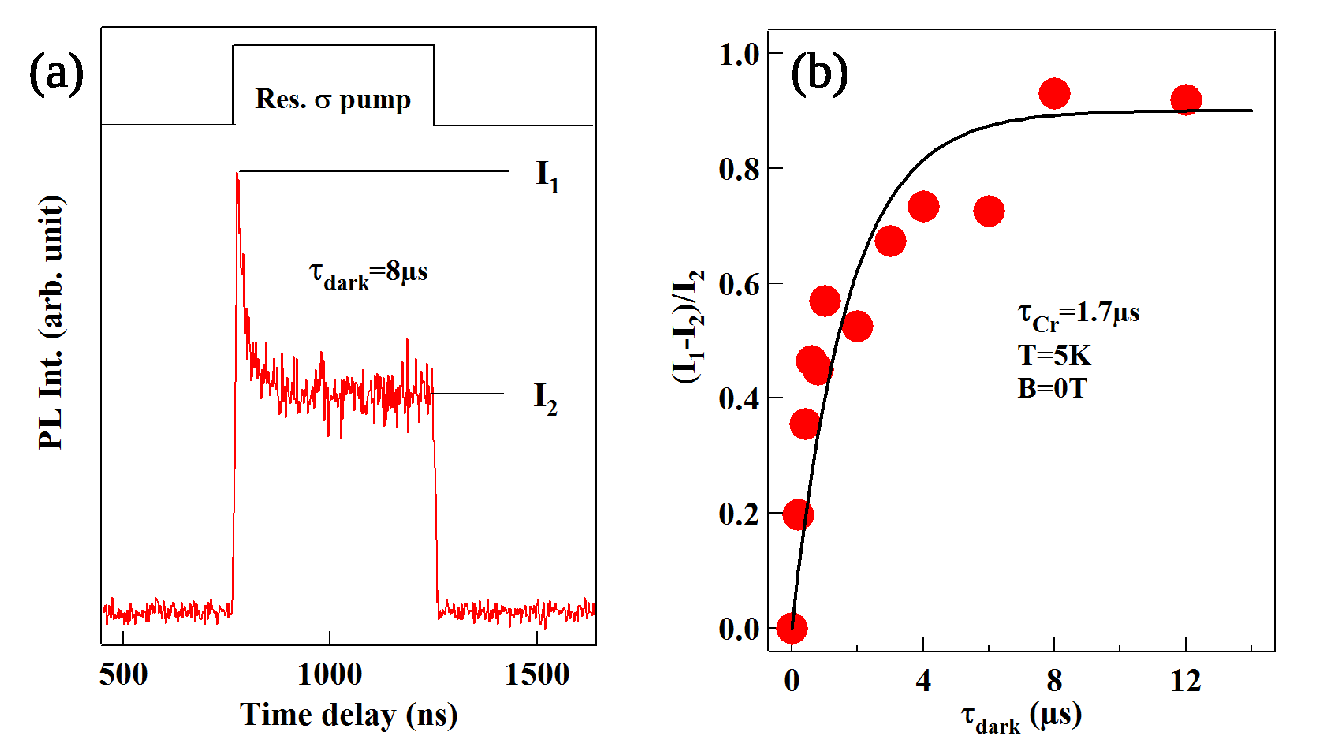
\includegraphics[width=12cm]{Pictures/RelaxDark.eps}
	\end{center}
	\caption{(a) Time evolution of the PL intensity of line (4) of X-Cr under resonant excitation on line (1) with a circularly polarized excitation pulse. (b) Evolution of the amplitude of the pumping transient $\Delta I/I_2$ as a function of the dark time between the excitation pulses. The black line is an exponential fit with a characteristic time $\tau_{Cr}=1.7$ $\mu$s}
	\label{RelaxDark}
	\end{figure}		
		
	From the time delay dependence of the amplitude of the transient, we deduce a Cr relaxation time $\tau_{Cr}\approx1.7$ $\mu$s at B$=0$ T and T$=5$ K. For such neutral QD and in the absence of optical injection of carriers, this spin relaxation is likely to be controlled by the spin-lattice interaction. Despite the large spin-phonon coupling expected for this magnetic atom with an orbital momentum and a strain induced spin splitting in the meV range~\cite{LafuenteCrQD}, the Cr spin relaxation time remains in the $\mu s$ range. This spin memory is long enough for a practical use of Cr in an hybrid spin nano-mechanical system and could even be improved in different QDs structures with weaker biaxial strain~\cite{LucienSFD}, lower magnetic anisotropy splitting and consequently less coupling with acoustic phonons~\cite{CaoSpinPhonCoupl}.
	
	The Cr spin-flip time found for a relaxation in the dark (microseconds range) is a lot longer than the one found under optical excitation (tens of nanosecond range, see Sec.~\ref{ResOptPump}). As shown in Sec.~\ref{hCrff}, the fast relaxation of the Cr under excitation is caused by the h-Cr efficient relaxation path. For Cr alone, the picture is quite different.
	
	After the pump pulse, the Cr spin state $S_z = -1$ has been partially emptied. During the dark time, it is repopulated from the states $S_z = 0$ and $S_z = +1$. The transfer is possible from the state $S_z = 0$ by a Cr spin flip mediated by the capture of a phonon. This one phonon mechanism is called direct mechanism, depending of the cube of the energy splitting between the states $\Delta_{i,j}$, with $i$ and $j$ the different Cr spin states.
	
	The direct mechanism is efficient for the transfer from $S_z = 0$, with $\Delta_{0, -1} \approx 2$ meV, but not for the transfer from $S_z = +1$, because $\Delta_{+1, -1} \approx 0$ meV. However, the states $S_z = +1$ and $S_z = -1$ are separated by two units of spin and close in energy. They are therefore mixed by the in-plane anisotropy term $E$~\cite{LafuenteCrQD}. This mixing can induce a transfer between the two states. Another possible source of transfer comes from two phonons mechanism: the system absorb a phonon, going from $S_z = +1$ to an excited state, and then relaxing by the emission of a phonon toward $S_z = -1$. Two processes exist: the Raman mechanism, using a virtual state as the excited state, or the Orbach mechanism, using an actual excited state of the system (e.g. $S_z = \pm2$).
	
	From this picture, we could expect two transition times: one between $S_z = 0$ and $S_z = \pm1$, driven by the direct mechanism, and one between $S_z = +1$ and $S_z = -1$, driven by the in-plane strain anisotropy and the two phonons mechanisms. However, Fig.~\ref{RelaxDark} shows only one time, suggesting that the second might occurs at a longer time scale.
%	
%	The population transfer can also come from the state $S_z = +1$. Since the splitting between $S_z = +1$ and $S_z = -1$ is negligible ($\Delta_{ij} \approx 0$), the transfer by a one phonon process is not efficient. However, two phonons process is possible: either the Orbach process, using an excited state as an intermediary, or the Raman process, using a virtual state. Two different times can therefore be expected: one for the one phonon process and one for the two phonons process. The $\mu$s time found in Fig.~\ref{RelaxDark} could then be the shorter of those two times only.

	\begin{figure}[h!]
	\begin{center}
		\includegraphics[width=14.8cm]{Pictures/RelaxHeat.png}
	\end{center}
	\caption{Comparison of the relaxation of the Cr spin after resonant pumping in the line (1) with (red) or without (blue) a probe pulse ($E_{probe} = 2070$ meV). (a) Time resolved PL of line (4) for a cross-circular resonant pump on line (1) with a probe pulse. (b) $\Delta I/I_2$ in function of the dark time $\tau_{dark}$ measured for the relaxation between the probe and the pump pulses (red) or between two pump pulses (blue). (c) Time resolved PL of line (4) for a cross-circular resonant pump on line (1) with no probe pulse.}
	\label{RelaxHeat}
	\end{figure}
	
	To analyze more in details the influence of non-equilibrium phonons on the relaxation of Cr, we recorded the amplitude of the pumping transient as a function of the delay after a probe pulse. Results are presented on Fig.~\ref{RelaxHeat} (b), with the data presented on Fig.~\ref{RelaxDark} (b) reported for reference. We observe the most intense transient for $\tau_{dark} \approx 0$ $\mu$s, more intense than the transient of the pump alone after a long dark time, due to the higher spin temperature created by the probe pulse. The transient normalized intensity decreases when the dark time is getting longer and Cr spin effective temperature decreases. However, after 20 $\mu$s of dark time, the transient normalized intensity is still decreasing. For the pump alone, the transient normalized intensity seems to stabilize for $\tau_{dark} \geq 8$ $\mu$s, at a lower value than the one measured with the probe ON. It shows that the Cr spin takes a long time to cool down in the dark, longer than the relaxation time measured with the pump alone. A $\tau_{Cr}$ of about 10 $\mu$s was found for the relaxation after the probe pulse.
	
	With the non-resonant probe, the system is brought to a non-equilibrium state distribution, at higher effective temperature than the lattice. This high effective temperature increases the population of the states $S_z = \pm1$. Therefore, during the dark time, the effective temperature of the Cr spin will decrease via transfers of population from $S_z = \pm1$ to $S_z = 0$. This relaxation would occur by the transfer mechanism presented above. The reduction of the transient with the dark time would then directly probe this transfer time. This would give us the two relaxation times we supposed above: one in the 10 $\mu$s range $\tau_{|\pm1\rangle \leftrightarrow |0\rangle}$, via a single phonon process, an one in the $\mu$s $\tau_{|\pm1\rangle \leftrightarrow |\mp1\rangle}$, via a two phonons process.
%	
%	This difference can be caused by the interaction with carriers injected by the probe or by the interaction with accoustic phonons, as discussed in Sec.~\ref{PhononHeat}. The effect lasting for more than 20 $\mu$s suggests that the cause of this change of dynamics might be the interaction with phonons, since the carriers have a short lifetime in the quantum dot (in the range of 0.1 ns).
%
	\section{Optical Stark effect on an individual Cr spin}
		
%		\subsection{Dressed atom picture and Autler-Townes splitting}	
	
	Optical Stark effect can be used to control the energy of a given state of a QD, using a high intensity optical field in resonance with a QD transition~\cite{CohOptSpectr,EmissionDressedExcBiexc}. It has been demonstrated that this control can also been achieved in QD doped with a single Mn atom~\cite{ClairStarkEffect}. In this case, each exciton-Mn level can be addressed and tuned individually. We propose in this section to demonstrate the same control possibility for a Cr embedded in a QD.
	
	When a laser is put on resonance with a QD transition, a coupling is created between the laser photons and the resonantly excited QD levels. The photons of the laser field are coherently absorbed by the ground state and emitted by the excited state at a Rabi flopping frequency $\Omega_r$, depending on the strength of the coupling between the laser field and the transition dipole. For a $n$ photons state of the control laser, the unperturbed states $|Cr\rangle \times |n\rangle$ and $|X-Cr\rangle \times |n-1\rangle$, degenerated at resonance, are no longer stationary solutions of the hamiltonian. Instead, stationary solutions are anti-linear (noted $|I, n\rangle$ in Fig.~\ref{StarkPres}) and linear ($|II, n\rangle$) combination of the unperturbed states, split proportionally to the Rabi flopping frequency $\Omega_r$. This splitting is called Autler-Townes splitting~\cite{AutlerTownes} and is well described by the dressed-atom picture. It can be exploited to control the coherent dynamics of a Cr spin~\cite{OptSignSpinSwitch, MnResSpinDyn}.
	
	\begin{figure}[h!]
	\begin{center}
		\includegraphics[width=13.5cm]{Pictures/AutlerTownes.png}
	\end{center}
	\caption{Illustration of the energy level of a Cr-doped quantum dot and formation of the dressed-states.}
	\label{StarkPres}
	\end{figure}

	In the dressed-atom formalism, the dressed state and the energy splitting are found using a quantum description of the QD levels and the laser field. We make the assumption that the Rabi splitting $\Omega_r$ and the laser detuning $\delta$ are small compared to the splitting between two PL lines of the quantum dot. We can then calculate the dressed states resulting from the interaction between the two levels of the QD addressed by the laser, noted $|G\rangle$ for the ground state and $|E\rangle$ for the excited state, and the resonant laser photons, neglecting the light-matter interaction of all the other levels. An illustration of such a system is given in Fig.~\ref{StarkPres} for $|G\rangle = |Cr\rangle$ and $|E\rangle = |X-Cr\rangle$, with $S_z = +1$ and $X_z = +1$.
	
	In the absence of coupling between the two considered states, the Hamiltonian of this two level system is written:
	\begin{align}
		{\cal H}_{AT}^{unpert} = \hbar \omega_L p p ^{\dagger} + \hbar \omega_{EG} |E\rangle \langle E|
	\end{align}
with $p$ (resp. $p^{\dagger}$) is the annihilation (resp. creation) operator for a photon in the mode $\omega_L$. The eigenstates of this system are $|G,n\rangle$, with the energy $\hbar n \omega_L$, and $|E,n\rangle$, with the energy $\hbar (\omega_{EG} + n \omega_L)$. Since the detuning $\delta = \omega_L - \omega_{EG}$ is many order of magnitude smaller than $\omega_L$ and $\omega_{EG}$, the energy level are grouped two by two. The energy levels are then organized in doublet, formed by the states $|G, n \rangle$ and $|E, n-1 \rangle$, split by $\delta$. The doublet are seperated from each other by $\hbar \omega_L$. The states are represented in Fig.~\ref{StarkPres} by $(Cr, n)$, $(XCr, n)$, $(Cr, n+1)$ and $(XCr, n+1)$, for $\delta = 0$.

	The light-matter interaction originates for the dipole interaction. In second quantification, in the rotating wave approximation, it is written:
	\begin{align}
		V \approx \hbar g (p |E\rangle \langle G| + p^{\dagger} |G\rangle \langle E|)
	\end{align}
with $g$ the electric dipole matrix element describing the couplig between the dipole of a QD transition and the mode $\omega_L$ of the electromagnetic field. The levels $|G, n \rangle$ and $|E, n-1 \rangle$ of a multiplet are coupled through stimulated emission ($p^{\dagger} |G\rangle \langle E|$) and absorption ($p |E\rangle \langle G|$) of a photon. The total hamiltonian write for a given $n$ photon state:
	\begin{align}
		{\cal H}_n =
		\begin{pmatrix}
			\hbar n \omega_L & \dfrac{\hbar \Omega_{r,n}}{2} \\
			\dfrac{\hbar \Omega_{r,n}}{2} & \hbar (\omega_{EG} + (n-1) \omega_L)
		\end{pmatrix}
	\end{align}
with $\Omega_{r,n} = g \sqrt{n}$ is the Rabi frequency and $\delta = \omega_L - \omega_{EG}$ the detuning of the laser. We write the mean energy of the $n$ photon state multiplet $E_n^0 = \frac{\hbar}{2}(\omega_{EG} + (2n - 1)\omega_L)$. The hamiltonian ${\cal H}_n$ becomes:
	\begin{align}
		{\cal H}_n = E_n^0 I_2 + \frac{\hbar}{2}
		\begin{pmatrix}
			\delta & \Omega_{r,n} \\
			\Omega_{r,n} & \delta
		\end{pmatrix}
	\end{align}
Diagonalizing the hamiltonian, we find the eigenstates $|I, n \rangle$ and $|II, n \rangle$ described at the beginning of this section:
	\begin{align}
		|I, n\rangle &= c |G, n\rangle - s |E, n-1\rangle \\
		|II, n\rangle &= c |G, n\rangle + s |E, n-1\rangle
	\end{align}
with $c = \sqrt{\dfrac{1}{2} \left(1 - \dfrac{\delta}{\Omega'_{r,n}}\right)}$ and $s = \sqrt{\dfrac{1}{2} \left(1 + \dfrac{\delta}{\Omega'_{r,n}}\right)}$, with $\Omega'_{r,n} = \sqrt{\Omega_{r,n}^2 + \delta^2}$ the generalized Rabi flopping frequency. We also find the corresponding energies and the splitting of the states:
	\begin{align}
		E_I &= E_n^0 - \frac{\hbar}{2} \Omega'_{r,n} \\
		E_{II} &= E_n^0 + \frac{\hbar}{2} \Omega'_{r,n} \\
		\Delta E_{I - II} &= \hbar \Omega'_{r,n}
	\end{align}

	At resonance ($\delta = 0$), $c = s = \sqrt{1/2}$. The states $|E, n-1 \rangle$ and $|G, n\rangle$ corresponding to the upper and lower levels of the transitions have then equal contribution to the dressed levels $|I, n\rangle$ and $|II, n\rangle$: the dressed states are entangled atom-field states.
	
%	At high excitation intensity, a strong coupling with the resonant laser field mixes the states with a Cr spin component $S_z=+1$ in the presence (X-Cr) or absence (Cr alone) of the exciton. In the ground state of the QD (Cr alone) two hybrid matter-field states are created (inset of Fig.~\ref{StarkPres}). Their splitting, $\hbar\Omega_r^{\prime}=\hbar\sqrt{\Omega_r^2+\delta^2}$, depends on the energy detuning of the laser $\hbar\delta$ and on its intensity through the Rabi energy $\hbar \Omega_r$~\cite{ExcDressStatesBeat}. It can be observed in the PL of all the X-Cr states associated with $S_z=+1$: the low energy bright exciton state $|S_z=+1,-1\rangle$ (line (4)) and the dark exciton $|S_z=+1,+2\rangle$ (line (5)), close in energy to the bright exciton and which acquires some oscillator strength through the exciton mixing induced by the electron-hole exchange interaction in a low symmetry QD~\cite{LafuenteCrQD}.
		
%		\subsection{Dressing of a Cr atom}

	\begin{figure}[h!]
	\begin{center}
		\includegraphics[width=14cm]{Pictures/StarkSplitDet.png}
	\end{center}
	\caption{(a) PL of QD2 X-Cr and configuration of excitation in the resonant optical control experiments. The inset illustrate the laser induced splittings in the ground and excited states for a $\sigma+$ excitation on $|S_z=+1\rangle$. (b) PL intensity maps of lines (5) and (4) for an excitation on (1) as a function of the detuning (top) and of the excitation intensity (bottom). The PL is produced by a second non-resonant laser.}
	\label{StarkSplitandDet}
	\end{figure}
	
	To observe the influence of a high power resonant laser on a QD doped with a single Cr atom, we used the optical configuration presented in Fig.~\ref{StarkSplitandDet}. A high intensity laser was put in resonance with the high energy transition, in $\sigma+$ polarization, exciting the state $S_z = +1$ in order to induce Autler-Townes splitting of this state. The splitting was observed using a non resonant excitation to generate PL by a transitions involving a third level and an optically dressed state.		

	The splitting observed experimentally is given by $\Omega'_{r,n}$, with $n$ the average number of photons of the laser excitation. This splitting depends on the Rabi splitting $\Omega_L = g\sqrt{n}$. Since $n$ is proportional to the laser power $P$, $\Omega_L$ is then proportional to $\sqrt{P}$. The PL of such a transition is split because, for instance, the emission from $|S_z = +1, -1 \rangle$ can occur toward any of the dressed states $(II, n)$ and $(I, n)$ as they contain the component of the $S_z = +1$ state. In our QD, such a splitting can be observed in the PL of all the X-Cr states associated with $S_z=+1$: the low energy bright exciton state $|S_z=+1,-1\rangle$ (line (4)) and the dark exciton $|S_z=+1,+2\rangle$ (line (5)), close in energy to the bright exciton and which acquires some oscillator strength through the exciton mixing induced by the electron-hole exchange interaction in a low symmetry QD~\cite{LafuenteCrQD}.
	
	\begin{figure}[h!]
	\fcapside{\caption{PL spectra of line (5) for an excitation on line (1) at (a) no detuning and max detuning in each direction, and (b) low and high power. The insets show the splitting of the PL doublet as a function (a) of the laser detuning and (b) of the excitation intensity. The fit is obtained with $\hbar\Omega_r = 100$ $\mu$eV.}\label{FitSplitDet}}	
	{\begin{center}
		\includegraphics[width=7cm]{Pictures/StarkFit.png}
	\end{center}}
	\end{figure}

	Both the line (4) and line (5) are split in the same fashion by an excitation on line (1), showing that all those states share a common ground state, and that the laser influence the energy of said ground state. The splitting measured on line (5) for a resonant excitation on line (1) is plotted as a function of the square root of the resonant laser intensity $P$ in Fig.~\ref{FitSplitDet} showing that, as expected for a two level system, it linearly depends on the laser field strength. The Rabi splitting can reach 150 $\mu eV$ at high excitation power. As the pump laser is detuned, the optically active transitions asymptotically approaches the original excitonic transitions where the remaining offset is the optical Stark shift.
	
	\begin{figure}[h!]
	\fcapside{\caption{PL of line (1) and (2) (high energy line) for a laser on resonance with the dark exciton state (5). Inset: PL intensity map of line (1) as a function of the laser detuning around (5).}\label{DarkExcSplit}}	
	{\begin{center}
		\includegraphics[width=6cm]{Pictures/StarkDark.eps}
	\end{center}}
	\end{figure}

	A resonant laser permits to address any spin state of the Cr and selectively shift its energy. For instance, as presented in Fig.~\ref{DarkExcSplit}, a $\sigma+$ excitation on the dark exciton state (5) induces a splitting of the high energy line (1) in $\sigma-$ polarization (state $|S_z=-1,-1\rangle$) without affecting the central line (2). This confirms that such resonant excitation can be used to tune the energy of $S_z=-1$ without affecting $S_z=0$.
	
	In this section, we have demonstrated the possibility to tune the Cr energy levels using optical Stark effect. The different Cr spin states can be addressed and controlled individually, without perturbing the other spin states. This open the possibility control the Cr spin state, which is a key step to use it in hybrid spin-mechanical system.
	
	\section*{Conclusion}
	
	The Cr spin dynamics was first observed using autocorrelation and crosscorrelation experiments, giving a relaxation time of the Cr spin $\tau_{Cr}$ under optical excitation in the 10 ns range.
	
	In order to analyse this dynamics in more details, we developed a resonant optical pumping experiment for the Cr spin. Several phonon related mechanisms were evidenced using this experiment. A fast transfer between $S_z = 0$ and $S_z = \pm1$ under excitation was demonstrated. This transfer was explained by h-Cr spins flip-flop similar to the one proposed for h-Mn in Sec.~III.2.3%~\ref{RelaxMech}
. It gives a hole-Cr relaxation time $\tau_{hCr}$ in the ns scale, in agreement with the time scale of the relaxation.

	Using resonant optical pumping, we also showed that the Cr spin dynamics is strongly affected by optically generated phonons. The possibility to heat the Cr spin through non-equilibrium phonons was demonstrated. A final proof of the effect could be given by depositing a thin metal layer on the back on the sample. A laser will then be able to excite phonons in it and inject them in the semiconductors without injecting any carriers.
	
	The relaxation of the Cr spin in the dark was also probed using resonant optical pumping. Two times were found, depending on the technique used to probe the relaxation. One was found in the $\mu$s range, while the other is about ten times higher. We proposed to explain those two times with two relaxation mechanism: a one phonon mechanism (direct mechanism) between $S_z = 0$ and $S_z = \pm1$, and a two phonon mechanisms (Raman or Orbach mechanisms) between $S_z = +1$ and $S_z = -1$. The states $S_z = \pm1$ are also mixed by the in-plane strain anisotropy term $E$.
	
	Several experiments can be done to test this last hypothesis and isolate those two transfer times. First, the direct mechanism could be probed using the relaxation in the dark of the state $S_z = 0$. A linearly polarized laser would excite both the states $S_z = +1$ and $S_z = -1$, and their populations would be transferred toward $S_z = 0$. The state of $S_z = 0$ would be probed in cross-linear configuration during the resonant excitation. The evolution of the pumping transient with the time between two pulses $\tau_{dark}$ would be a measure of the transfer between $S_z = 0$ and $S_z = \pm1$ via the direct mechanism.
	
	The transfer mechanism between $S_z = +1$ and $S_z = -1$ could be probed using other experiments. First, probing the Cr spin relaxation in the dark under magnetic field would shows whether this relaxation is driven by $E$ or by the two phonons mechanisms: two levels need to be almost degenerated to be efficiently coupled by $E$. Therefore its effect should disappear quickly in magnetic field, whereas the effect of the two phonons mechanism would need a higher magnetic field to disappear. Probing the evolution of $\tau_{Cr}$ in temperature would confirm the role of phonons in the transfer mechanism. The Raman mechanism depends on $T^7$. It should therefore be inefficient at low temperature, and become quickly important as the temperature rises.
	
	We finally demonstrated the possibility to control the Cr spin state using optical Stark shift. It is possible to independently tune each Cr spin state. This energy tuning is particularly interesting for the control of the Cr spin states $S_z=\pm1$. These states could be efficiently mixed by applied weak anisotropic in-plane strain through a fine structure term of the form $E(S_x^2-S_y^2)$~\cite{LafuenteCrQD}. A relative shift of the energy of $S_z=+1$ or $S_z=-1$ by a resonant optical excitation would affect their coupling and consequently the Cr spin coherent dynamics.
	
\printbibliography

\end{document}